\subsection{Data Collection}

Data collection is a crucial step in any research. When conducting a text analysis, there is more often than not a need to collect data from the internet. The difficulty of this task can vary depending on the source of the data. For example, data from social media platforms or research portals is often easier to collect than data from websites. This is because these platforms often provide APIs that allow developers to collect data. On the other hand, other websites do not always provide APIs. In such cases, researchers may have to resort to webscraping. Webscraping is a method of automatically extracting, combining and saving data from websites. The paper uses webscraping to collect data from scamalert.sg.

\subsubsection{Scamalert}

Scamalert is a singaporean website run by the National Crime Prevention Council (NCPC), which is a non-profit organization that is committed promoting public awareness and concern about crime and to propagate the concept of self-help in crime prevention.~\citep{ncpc} Scamalert contains educational sources to help people protect themselves from scams as well as provide information about acting after falling victim to a scam.

Most relevant to this paper is the section "Scam Stories". Persons who experience a crime can share their stories on the website. The stories can be sent anonymously and are published on the website. The stories are well-formatted, all containing a title, date, category, and the story itself.

Scamalert does not provide an API to access the stories. Therefore, webscraping was used to collect the data. 

\subsubsection{Webscraping}

The webscraping process was done using four libraries in Julia. Julia is a contemporary programming language that is designed for high-performance computing which is favored among data scientists. % TODO: Add citation
The four libraries in use were:

\begin{itemize}
    \item HTTP.jl\footnote[0]{\url{https://juliaweb.github.io/HTTP.jl/stable/}}: A library for making HTTP requests and handling responses 
    \item Gumbo.jl\footnote[1]{\url{https://github.com/JuliaWeb/Gumbo.jl}}: A library for parsing HTML documents
    \item Cascadia.jl\footnote[2]{\url{https://docs.juliahub.com/Cascadia/Pq6Fi/0.4.0/}}: A library for querying HTML documents using CSS selectors
    \item JSON.jl\footnote[3]{\url{https://docs.juliahub.com/JSON/uf6oy/0.21.0/}}: A library for parsing JSON documents
\end{itemize}

The first step of webscraping is figuring out the structure of the website to find an efficient way of scraping the data. Fortunately, the website was well-structured. The \texttt{/stories} directory contains all the pages with stories. The stories are paginated, with each page containing data about 6 stories. The pages contained a lot of metadata about the stories, but the most important were the following: title, date, category, URL and description of the story. The story itself is not included in the page. 

\begin{figure}
    \centering
    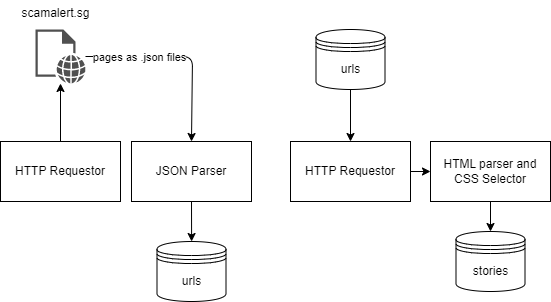
\includegraphics[width=0.4\textwidth]{resources/webscraper.drawio.png}
    \caption{Webscraping process.}
    \label{fig:webscraping}
\end{figure}

This meant that the webscraping needed to be done in two steps. The first step was to collect the metadata of the stories. This was done through POST requests using HTML.jl and then parsing them into .json files. The second step was to collect the stories themselves. By extracting the URLS from the .json, the pages containing the stories were downloaded as .html files, which were parsed using Gumbo.jl and Cascadia.jl, and the stories were extracted. The process is illustrated in figure \ref{fig:webscraping}.

The data was collected on the 10th of July 2023. On the first step, a total of 590 pages were scraped, containing a total of 3536 stories. It was observed later in the process that the requests did not contain the category of the scams. This was not remedied as the category was not considered for the analysis.

The second step retrieved 3495 stories, which is 41 stories less than expected. The process of scraping was logged. The logs have shown that there were 41 errors. The errors were not caused by connectivity issues, but rather by selector issues encountered by Cascadia.jl. Upon further investigation, it was found that the cause of the errors was the HTML documents themselves. The retrieved HTML documents contained an error that is likely caused by the website host deleting the story.

After the webscraping step, a decision was made to switch to Python as the choice for a programming language.

\subsubsection{Data Preprocessing}

Another important step of data analysis is the prepocessing of data. Data preprocessing can be defined as the cleaning of data and parsing it into a format that is suitable for further processing. An example of this is the removal of non-english stories, since the analysis aims to only consider stories written in english. There were a total of 5 non-english stories. The stories were removed from the dataset.

Since the aim is to do a text analysis, it is necessary to use natural language processing (NLP). NLP combines aritificial intelligence and linguistics to enable "understanding" of content. NLP is critical for topic models, as it is used to bring the text into a format that is suitable for topic modeling. Preprocessing also increases the accuracy of both topic models and sentiment analyses.~\cite{haddi2013role}\cite{chauhan2021topic}

\subsubsection*{Preprocessing for Topic Modeling}

The preprocessing step for the topic model is illustrated in the following figure (figure \ref{fig:preprocessing_topic_modeling}):

\begin{figure}[h]
    \centering
    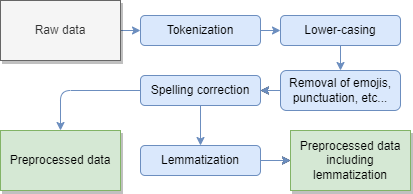
\includegraphics[width=0.6\textwidth]{resources/preprocessing_topic_modeling.png}
    \caption{Data preprocessing for topic modeling. Two datasets are produced, one is with lemmatization and one is without.}
    \label{fig:preprocessing_topic_modeling}
\end{figure}

The preprocessing was done using the Natural Language Toolkit (NLTK) library. Using NLTK, the text was tokenized, brought to lower-case, stripped off of punctuation, numbers, stopwords and emojis. Then the data was split into two sets: a set with lemmatizing and a set without lemmatizing. Lemmatizing is the process of reducing words to their root form. For instance, the word "writing" is reduced to "write". While lemmatization is a common preprocessing step, the decision to split the data was made on the basis of the claim that lemmatization correlates negatively with human interprability of english topic models.~\cite{schofield2016comparing} An example of a sentence that is preprocessed is illustrated in the table below:


\begin{table}[h]
    \centering
    \begin{tabular}{cc}
        Original & Preprocessed \\ \hline
        I was scammed by a fake website. & scam fake website \\
        \\
        Original & Preprocessed (without lemmatization) \\ \hline
        I was scammed by a fake website. & scammed fake website \\
    \end{tabular}
    \caption{Example of a preprocessed sentence. The word "scammed" was not returned to its root form in the second table.}
    \label{tab:preprocessing}
\end{table}

Additionally, the spellchecker library for Python was used to correct spelling mistakes. The spell-correction is based on edit distance, so it is not context aware. This does not include grammatical errors. It is not a usual practice to correct for spelling errors in topic modeling. However, since the data set consists of stories written by users, there is a high chance of spelling errors. A distance of 1 was used, which means that the spellchecker will only correct words that are one edit away from a word in the dictionary. This is the recommendation of the authors.~\cite{spellchecker2023}

Initially, the TextBlob library was used to correct spelling errors. However, upon discovering that the library has a 70\% accuracy ~\cite{loria2018textblob}, the decision was made to switch to the spellchecker library. The authors of the spellchecker library do not have a statement about the accuracy, but on the basis of some back-of-the-envelope testing, it seemed to be far more accurate.

\begin{figure}[h]
    \centering
    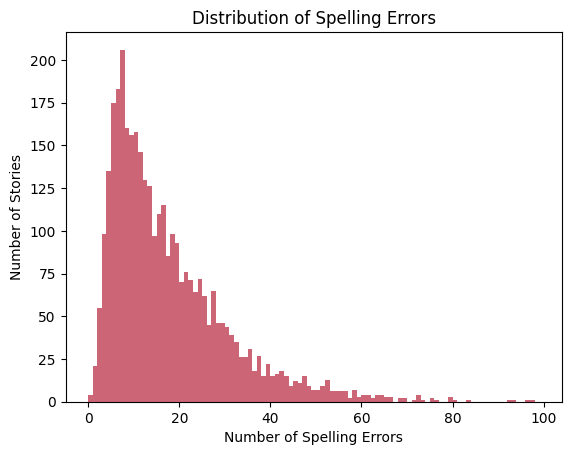
\includegraphics[width=0.8\textwidth]{resources/spelling_mistakes_distribution.png}
    \caption{Distribution of spelling errors}
    \label{fig:spelling_error_distribution}
\end{figure}


A spelling error analysis revealed that there was a total of 61070 spelling mistakes in 505672 words ($\approx 12\%$). The mean error was $\approx17$ errors per story. The median error was 13 errors per story. The conclusion was that the spelling errors were significant enough to warrant correction. The caveat is that the spellchecker library is not context-aware, it uses edit-distance algorithms to correct spelling errors. This means that it is possible to get corrections that false positives. For example, if the word "fraud" was mispelled as "faurd", it could be corrected to "found". However, it seemed that the benefits of correcting spelling errors outweighed the risks. The idea was that a false positive would appear too infrequently to have an impact on the analysis, while a true positive would contribute to the accuracy of it.

\subsubsection*{Preprocessing for Sentiment Analysis}

The preprocessing for sentiment analysis was simpler than that of topic modeling. The text was sentence-tokenized then split into two datasets, one with spelling correction and one without. Extensive preprocessing will likely remove lexical features that are important for sentiment analysis. Emojis and negations are simple examples of this. This will be elaborated further in the section about sentiment analysis.

\begin{figure}[h]
    \centering
    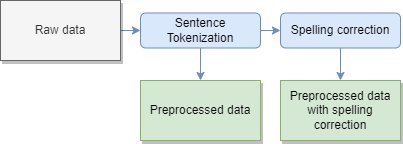
\includegraphics[width=0.6\textwidth]{resources/preprocessing_sentiment_analysis.png}
    \caption{Data preprocessing for sentiment analysis. Two datasets are produced, one is with spelling correction and one is without.}
    \label{fig:preprocessing_sentiment_analysis}
\end{figure}